\chapter{Gradient Descent}

\section{Introduction}
Gradient Descent is a \tc{first-order iterative optimization algorithm} for finding local minimum points of a differentiable function. It's commonly used in machine learning and optimization problems (e.g., matrix factorization, neural networks), especially when dealing with non-convex cost functions that don't have a closed-form solution.
% GD is an iterative optimization algorithm.
\section{General Template of GD-Style Algorithms}
% GD is an iterative optimization algorithm.\\ \\
Let the function being optimized be dependent on the weight vector $\tc{w}$. We now wish to find the optimal value of $\tc{w}$ so that the function in consideration is minimized (since its the loss function which we generally are trying to optimise in ML). GD-style algorithms helps us in finding that. The general flow of such algorithms is as follows:
\begin{itemize}
  \item Initialize {\tc{w}} (e.g. ${\tc{w}} = \Vec{0}$)
  \item Repeat
        \begin{itemize}
          \item Choose a descent direction (directions of fastest decrease)
          \item Choose a step size
          \item Update ${\tc{w}}$
        \end{itemize}
  \item Exit repeat loop when certain stopping criterion is met. Some common stopping criterion include  (where $t$ represents a time step)
        \begin{itemize}
          \item $|| \nabla L(w_{t}) ||_{2} < \epsilon$
          \item $|| {w_{t+1} - w_{t}} ||_{2} < \epsilon$
        \end{itemize}
\end{itemize}
\section{Algorithm of Gradient Descent}
The flow for the Gradient Descent algorithm keeping in the mind the template above is:
\begin{itemize}
  \item $\tc{w} \leftarrow \tc{w}_{0}$ : Initialisation can be done in various ways such as zero initialisation ($w_{0} = \Vec{0}$), randomly sampled Gaussian etc.
  \item For the iterative part, we use the following values :
        \begin{itemize}
          \item Direction : $- \nabla L(\tc{w}_{t})$
          \item Step size (Learning Rate) : $\alpha > 0$ is a hyperparameter
          \item Update : $\tc{w}_{t+1} \leftarrow \tc{w}_{t} - \alpha \nabla L(\tc{w}_{t})$
        \end{itemize}
  \item Some common stopping criteria used among others are:
        \begin{itemize}
          \item $|| \nabla L(w_{t}) ||_{2} < \epsilon$
          \item $|| w_{t+1} - w_{t} ||_{2} < \epsilon$
        \end{itemize}
\end{itemize}

\begin{algorithm}[H]
  \caption{Gradient Descent Algorithm with Epochs}
  \label{algo:gradient_descent_epochs}
  \SetKwInOut{Input}{Input}
  \SetKwInOut{Output}{Output}
  \Input{Initial weight vector $w_0$, step size $\alpha > 0$, tolerance $\epsilon > 0$, maximum number of epochs $N_{\text{max}}$}
  \Output{Optimal weight vector $w^*$}
  $w \gets w_0$\;
  \For{$t \gets 1$ \KwTo $N_{\text{max}}$}{
  Compute gradient direction: $\nabla L(w)$\;
  Update: $w \gets w - \alpha \nabla L(w)$\;
  \If{$||\nabla L(w)||_{2}^{2} \leq \epsilon$}{
  \tc{break}\;
  }
  }
  \Return{$w^* = w$}
\end{algorithm}

\subsection{Why the name Gradient Descent ?}
The name Gradient Descent is made of two parts:
\begin{itemize}
  \item \tc{Gradient} :  Gives us the direction of fastest increase in function L
        \begin{equation*}
          \nabla L(w) =
          \begin{bmatrix}
            \frac{\partial L(w)}{\partial w_{1}} \\
            \frac{\partial L(w)}{\partial w_{2}} \\
            \vdots                               \\
            \frac{\partial L(w)}{\partial w_{d}} \\
          \end{bmatrix}
        \end{equation*}
  \item \tc{Descent} : Since we update in the direction of fastest decrease in L
\end{itemize}
\section{GD for the 1-D case and Linear Regression}
\begin{figure}[h]
  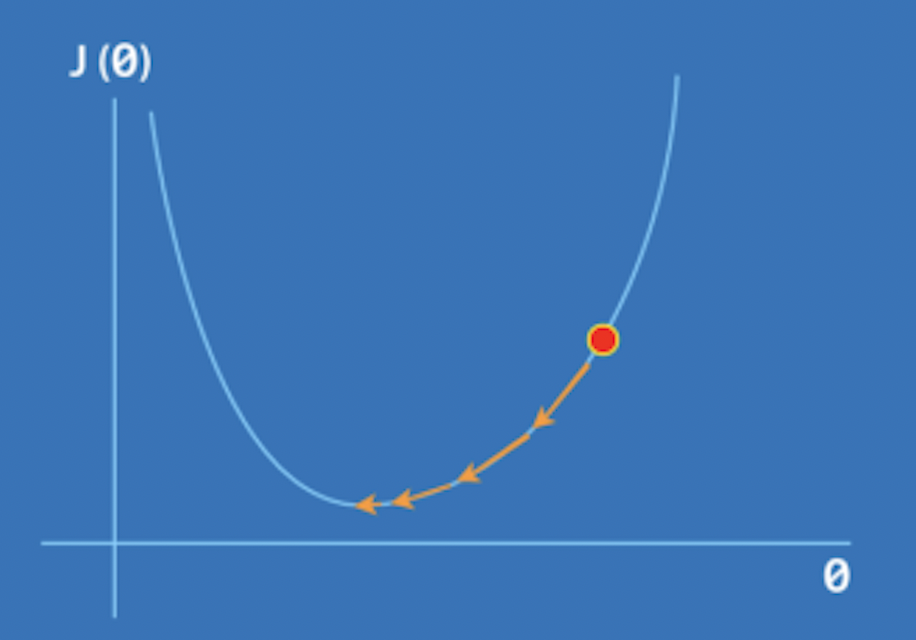
\includegraphics[width=8cm]{images/10.png}
  \centering
\end{figure}

The overall representation of Gradient Descent in linear regression would take on a similar form as given in the plot above, and given that the step size governs the speed and feasibility of convergence, it leads us to inquire about the following matters:

\subsection{What if the step size is too small?}

The plot obtained with very small step size would look something like the plot given below
\begin{figure}[H]
  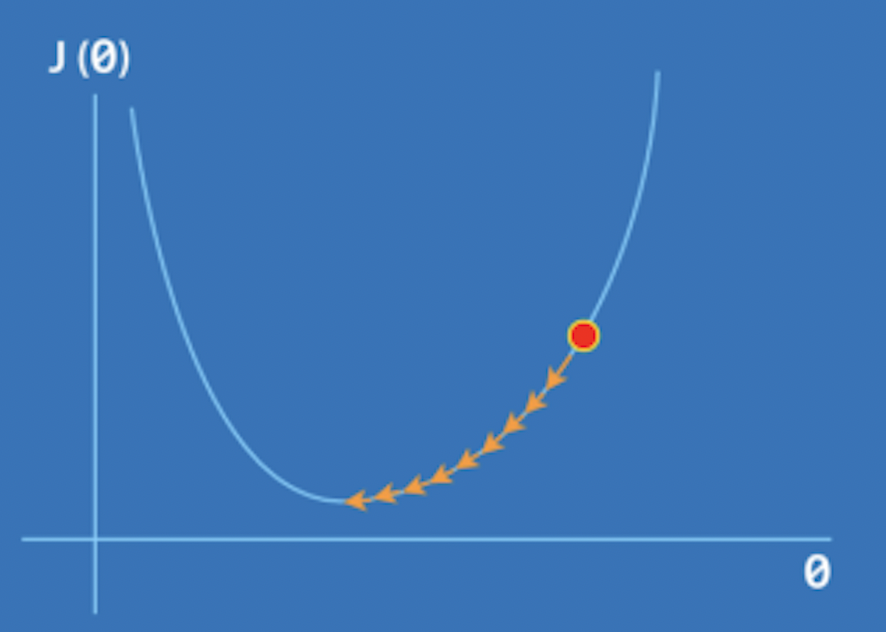
\includegraphics[scale=0.3]{images/11.png}
  \centering
\end{figure}

From the plot, we can conclude that the loss will take very long to converge since we only update by a small value each time. This may also result in never reaching the optimal point if we train using a (fixed) maximum number of epochs.

\subsection{What if the step size is very large?}

The plot obtained with very large step size would look something like the plot given below
\begin{figure}[H]
  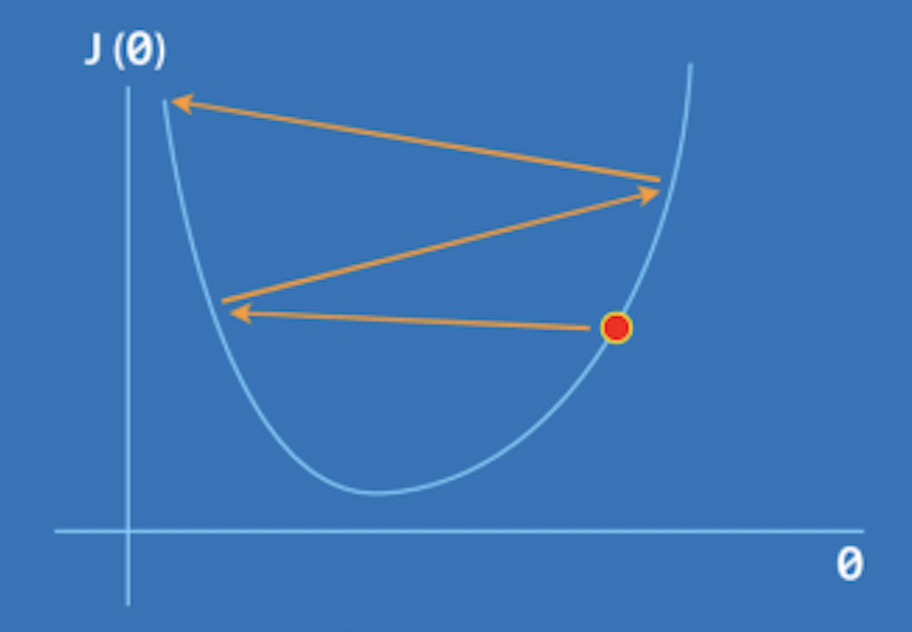
\includegraphics[scale=0.3]{images/12.png}
  \centering
\end{figure}

Clearly in this case the curve will take longer to converge or in the worst case may diverge as seen above.

\section{Weight update rule in GD for linear regression}

The formula for update of $\tc{w}$ is,
\begin{equation}
  \label{eqn:1}
  \tc{w} \leftarrow \tc{w} -\alpha \nabla L(\tc{w})
\end{equation}

\tc{Unregularized Loss}:
\begin{equation}
  L(\tc{w}) = \frac{1}{N}\sum_{i}^N(y_{i} - \tc{w}^{T}\tc{x}_{i})^2
\end{equation}
\begin{equation}
  L(\tc{w}) = \frac{1}{N}\sum_{i}^N(y_{i} - \hat{y_i})^2
\end{equation}
\begin{equation}
  \label{eqn:3}
  \frac{\partial L(\tc{w})}{\partial \tc{w}} = -\frac{2}{N} \sum_{i}^N(y_{i} - \hat{y_{i}})\tc{x}_i = \frac{2}{N} \sum_{i}^N(\hat{y_{i}} - y_{i})\tc{x}_i
\end{equation}

$$\boxed{\tc{w}^{t+1} \leftarrow \tc{w}^{t} - \alpha \frac{2}{N}\sum_{i}^N([\tc{w}^t]^T\tc{x}_i - y_{i})\tc{x}_i}$$

\section{Different Variants of Gradient Descent}
\subsection{(Full) Gradient Descent}

Here, we find the gradient of loss function over the entire training dataset. Our gradient update formula in this case is :
$$
  \tc{w} \leftarrow \tc{w} -\alpha \nabla L(\tc{w}, \D_{train})
$$

The training data can be very large in many applications of ML with millions of data points. Hence, it seems wasteful to compute the full loss function over the entire training set in order to perform only a single parameter update. Hence, we usually use other variations of GD which helps us in avoiding this computationally expensive step of finding gradient of loss over entire data every time.

\subsection{Stochastic Gradient Descent(SGD)}

In this modification of GD, rather than finding gradient of loss over entire training set, we find loss over only single instance of training data that is picked randomly and we update \tc{w} based on the gradient for this loss,
$$\tc{w} \leftarrow \tc{w} - \alpha \nabla L(\tc{w}, \D_{random})$$
where $\D_{random}$ = \{($x_{i}$,$y_{i}$)\}, $(x_{i},y_{i}) \rightarrow$ randomly sampled point in $\D_{train}$\\
Now the issue with this version is that there is a lot of noise in the convergence path of the loss function, as a single data point is not representative of entire data set and this leads to lot of fluctuations in computed gradient. Outliers can lead to training instability in this
case. For example, training may stop prematurely, if for a certain point gradient becomes
zero.

\subsection{Mini Batch Gradient Descent}
In this version of GD, we try to find the best of both the worlds of GD and SGD by using the gradient of loss computed over only a batch (small subset) of original data set. This helps not only in faster gradient calculation but also is less noisier as batch is still a better representative than a single instance used in SGD.
$$
  \tc{w} \leftarrow \tc{w} - \alpha \nabla L(\tc{w}, \D_{batch})
$$

where $\D_{batch}$ = $\{(x_{i},y_{i})\}_{i = 1}^{\mathbb{B}}$, $\mathbb{B} = $batch size\\
Here $\mathbb{B}$ is a hyper parameter. We should know that larger $\mathbb{B}$ is more stable as we approach close to GD and smaller $\mathbb{B}$ is less stable as we move closer to SGD, so the onus lies on us to find that optimal $\mathbb{B}$ that can help us gain the benefit of both the worlds. Also, note that it is a common convention to use $\mathbb{B} = 16,32,64 ...$ usually a power of 2. This method is an improvement over SGD, as it enhances training
stability. Batches are randomly sampled during each epoch.

\section{Probabilistic View of Linear Regression}

For training data $\D = \{(x_{i}, y_{i})\}^{\text{n}}_{i=1}$. Let the target $y_{i}$ have some noise defined as: $$y_{i} = f(x_{i}) + \epsilon_{i}, \qquad \epsilon_{i} \sim \mathcal{N}(0,\sigma^{2})$$
$\epsilon_{i^{'}s}$ are independent and identically distributed (\tc{i.i.d.}), 0 mean Gaussians with the some variance $\sigma^{2}$.(Cov($\epsilon_{i}$, $\epsilon_{j}$) = 0 for all $j \neq i$).
So basically now we can get the following interpretation of data,

\begin{align*}
  \textit{y}_i                               & = f(\textit{x}_i) + \epsilon_i                                                                                                               \\
  \implies \textit{y}_i                      & = \tc{w}^T\textit{x}_i + \epsilon_i                 &                                                                                        \\
  \implies \textit{y}_i                      & \sim \mathcal{N}(\tc{w}^{T}\textit{x}_i , \sigma^2)                                                                                          \\
  \implies \text{P}(y_{i}\mid x_{i}, \tc{w}) & \sim \mathcal{N}(\tc{w}^{T}x_{i} \sigma^{2}),       & \hfill \text{[where }\text{P}(y_{i}\mid x_{i}, \tc{w}) \text{ is likelihood function]}
\end{align*}

For training data $\D = \{(\mathit{x}_{i}, \mathit{y}_{i})\}^{\text{n}}_{i=1}$,
$$
  \text{P}(y_{1}, y_{2}, \ldots, y_{n}\mid x_{1}, x_{2}, \ldots, x_{n}, \tc{w}) = \prod_{i}\text{P}(y_{i}\mid x_{i}, \tc{w})
$$
where $y_{i}$'s are conditionally independent given $x_{i}$'s.

$$
  \implies \log\text{P}(y_{1}, y_{2}, \ldots, y_{n}\mid x_{1}, x_{2}, \ldots, x_{n}, \tc{w}) = \sum_{i}\text{log P}(y_{i} \mid x_{i}, \tc{W})
$$

Note, here we can use log likelihood instead of likelihood because of following reasons,
\begin{itemize}
  \item Does not change the maxima or minima of function as log is monotonic function
  \item Mathematical convenience
  \item Computational convenience as it is easier to add many small values than to multiply them as they might underflow if multiplied
\end{itemize}